\documentclass[11pt,a4paper]{ctexart}

\usepackage[margin=2.2cm]{geometry}
\usepackage{amsmath,amssymb,mathtools}
\usepackage[dvipsnames]{xcolor}
\usepackage{graphicx}
\usepackage{booktabs}
\usepackage{array}
\usepackage{enumitem}
\usepackage{hyperref}
\usepackage{needspace}
\usepackage[most]{tcolorbox}
\usepackage{tikz}
\usepackage{listings}
\usetikzlibrary{arrows.meta,calc,matrix,positioning,fit,decorations.pathreplacing}

\graphicspath{{../images/}}

\hypersetup{
  colorlinks=true,
  linkcolor=MidnightBlue,
  urlcolor=RoyalBlue!60!black
}

\setlist[enumerate]{itemsep=0.35em, topsep=0.45em}
\setlist[itemize]{itemsep=0.35em, topsep=0.45em}

\tcbset{
  commonbox/.style={
    enhanced,
    breakable,
    boxrule=0.8pt,
    arc=2mm,
    left=1.5mm,
    right=1.5mm,
    top=1mm,
    bottom=1mm,
    colback=white
  }
}

\newtcolorbox{problemblock}{commonbox,colframe=BrickRed!65!black,colback=BrickRed!4,title=背景问题,fonttitle=\bfseries}
\newtcolorbox{intuitionblock}{commonbox,colframe=RoyalBlue!70!black,colback=RoyalBlue!4,title=朴素直觉,fonttitle=\bfseries}
\newtcolorbox{definitionblock}{commonbox,colframe=Purple!60!black,colback=Purple!4,title=定义,fonttitle=\bfseries}
\newtcolorbox{mathblock}[1]{commonbox,colframe=Purple!60!black,colback=Purple!4,title=#1,fonttitle=\bfseries}
\newtcolorbox{codeblock}{commonbox,colframe=ForestGreen!60!black,colback=ForestGreen!4,title=代码对应,fonttitle=\bfseries}
\newtcolorbox{questionblock}{commonbox,colframe=Orange!75!black,colback=Orange!5,title=新手提问,fonttitle=\bfseries}
\newtcolorbox{keypointblock}{commonbox,colframe=black!65,colback=black!3,title=这一页该记住,fonttitle=\bfseries}

\lstset{
  basicstyle=\ttfamily\small,
  breaklines=true,
  columns=fullflexible,
  keywordstyle=\color{Purple!70!black}\bfseries,
  commentstyle=\color{gray!70!black}\itshape,
  stringstyle=\color{ForestGreen!50!black},
  showstringspaces=false,
  language=Python,
  frame=single,
  rulecolor=\color{black!20},
  framesep=2pt,
  xleftmargin=0.5em
}

\newcommand{\vect}[1]{\boldsymbol{#1}}
\newcommand{\mat}[1]{\boldsymbol{#1}}
\newcommand{\softmax}{\operatorname{softmax}}

\title{零基础读懂 Self-Attention\\\large 从“词互相看一眼”到 Query--Key--Value 公式}
\author{}
\date{2026 年 4 月 22 日}

\begin{document}

\maketitle

\begin{center}
\small
基于 Lena Voita 的 NLP Course 中
\href{https://lena-voita.github.io/nlp_course/seq2seq_and_attention.html#self_attention}{Self-Attention: the ``Look at Each Other'' Part}
小节整理。本文是中文零基础讲义，不是逐句翻译。
\end{center}

\tableofcontents
\newpage

\section{这一节到底在解决什么}

\begin{problemblock}
我们已经知道，机器不能直接处理“词”，它处理的是向量。
一句话进入 Transformer 以后，会先变成一排 token 向量。
现在的问题是：\textbf{每个 token 怎样吸收同一句话里其它 token 的信息？}
\end{problemblock}

例如一句话是：

\begin{center}
\textit{The animal did not cross the street because it was tired.}
\end{center}

里面的 \textit{it} 到底指谁？单看 \textit{it} 自己几乎看不出来。
它必须回头看 \textit{animal}、\textit{street}、\textit{tired} 等词，再根据整句话的语境更新自己的表示。

\begin{intuitionblock}
Self-attention 的核心直觉很短：
\textbf{一句话里的每个 token 都看同一句话里的其它 token，收集上下文，再更新自己。}
这里的 “self” 不是“只看自己”，而是“同一组表示内部互相看”。
\end{intuitionblock}

Lena Voita 的原文把这部分叫作模型中 token ``look at each other'' 的部分。
这句话很重要：它不是把整句话压成一个单独向量，而是让每个位置都得到一个新的、带上下文的向量。

\begin{figure}[htbp]
  \centering
  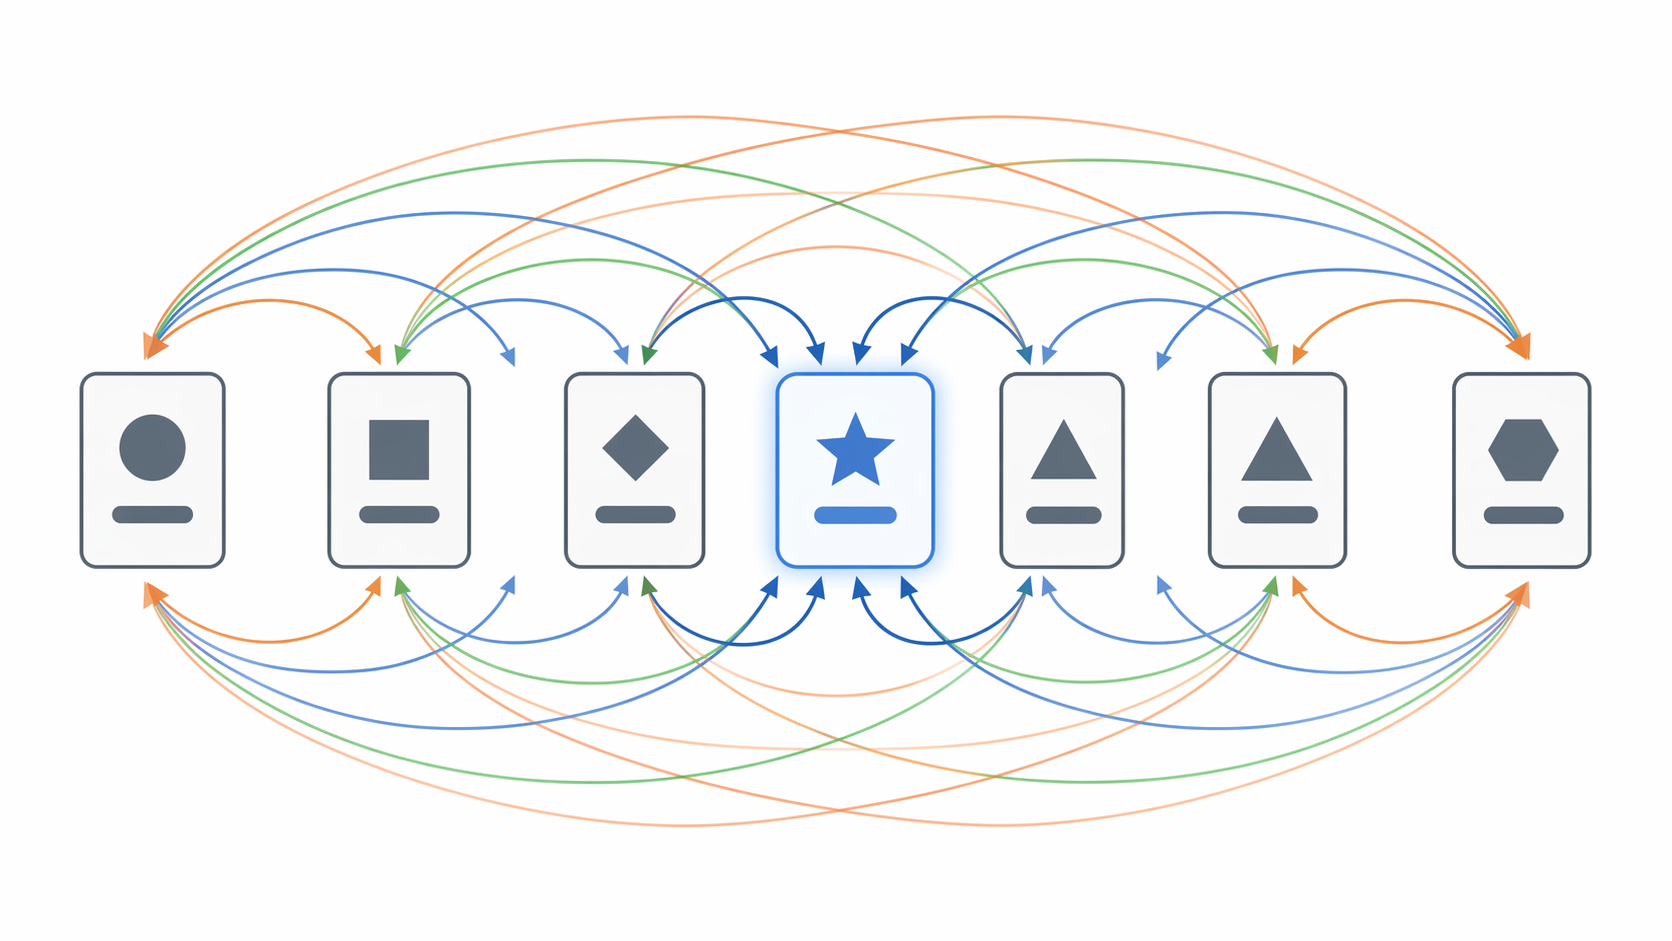
\includegraphics[width=0.92\linewidth]{self_attention_parallel.png}
  \caption{Self-attention 的视觉直觉：同一句话里的 token 并行地互相查看。图内没有写词，是为了把注意力放在“连接关系”本身。}
  \label{fig:self-attention-parallel}
\end{figure}

\section{新的讲解原则}

本讲义按四层来解释，每层都只推进一个问题：

\begin{enumerate}[label=\textbf{\arabic*.}]
  \item \textbf{背景问题}：为什么需要 self-attention？
  \item \textbf{朴素直觉}：token 之间怎样“互相看”？
  \item \textbf{数学表达}：Query、Key、Value 和公式每一项是什么意思？
  \item \textbf{代码对应}：真实代码里通常会出现哪些张量形状？
\end{enumerate}

\begin{keypointblock}
如果你第一次学 attention，不要先背公式。
先记住：\textbf{谁在问、问谁、拿回什么信息}。
公式只是把这三件事写成矩阵乘法。
\end{keypointblock}

\section{新手最该问的 5 个问题}

\begin{enumerate}[label=\textbf{Q\arabic*.}]
  \item Self-attention 和普通 attention 的差别是什么？
  \item “每个 token 看其它 token” 到底是怎么计算出来的？
  \item Query、Key、Value 为什么要分成三种角色？
  \item 公式 \(\softmax(QK^\top/\sqrt{d_k})V\) 每一项在做什么？
  \item 这和真实 Transformer 还差哪些部件？
\end{enumerate}

\section{Q1：Self-Attention 和普通 Attention 差在哪里}

\begin{questionblock}
普通 attention 也是“看别处”，self-attention 也是“看别处”。
那为什么要多一个 “self”？
\end{questionblock}

\begin{definitionblock}
\textbf{Attention} 是一种“按相关程度汇总信息”的机制。
如果被看的对象来自另一组表示，例如 decoder 当前状态去看 encoder 输出，这通常叫 encoder--decoder attention。

\textbf{Self-attention} 是同一组表示内部做 attention。
例如 encoder 某一层里的所有 token 状态彼此查看，或者 decoder 某一层里已经允许查看的位置彼此查看。
\end{definitionblock}

更直白地说：

\begin{center}
\begin{tabular}{>{\raggedright\arraybackslash}p{0.28\linewidth} >{\raggedright\arraybackslash}p{0.60\linewidth}}
\toprule
机制 & 直觉 \\
\midrule
普通 attention & 我这一组表示，去看另一组表示。\\
self-attention & 我们这一组表示，在组内互相看。\\
\bottomrule
\end{tabular}
\end{center}

在 Transformer encoder 里，输入句子的所有 token 同时进入一层。
这一层里的每个 token 都有机会看所有 token，包括自己。
看完以后，每个 token 的向量都会变成“带上下文的新向量”。

\section{Q2：Token “看其它 token” 是怎么计算的}

\begin{questionblock}
“看一眼”听起来像比喻。
模型真正能做的只有加减乘除。
这个“看”到底对应什么计算？
\end{questionblock}

\begin{intuitionblock}
先想一个极简版本。
每个 token 都拿自己的向量去和其它 token 的向量做相似度比较。
越相似，说明越应该多看一点；越不相关，就少看一点。
最后把所有 token 的信息按权重加起来。
\end{intuitionblock}

这一过程可以拆成三步：

\begin{enumerate}[label=\textbf{\arabic*.}]
  \item \textbf{打分}：当前 token 和每个候选 token 算一个相关分数。
  \item \textbf{归一化}：用 softmax 把分数变成一排权重，权重全为正且加起来等于 1。
  \item \textbf{汇总}：用这些权重对候选 token 的信息做加权求和。
\end{enumerate}

\begin{mathblock}{极简版公式}
设第 \(i\) 个 token 的旧向量是 \(\vect{x}_i\)，第 \(j\) 个 token 的旧向量是 \(\vect{x}_j\)。
如果暂时不区分 Query、Key、Value，可以写成：
\[
  s_{ij} = \vect{x}_i \cdot \vect{x}_j,
  \qquad
  a_{ij} = \frac{\exp(s_{ij})}{\sum_{r=1}^{n}\exp(s_{ir})},
  \qquad
  \vect{z}_i = \sum_{j=1}^{n} a_{ij}\vect{x}_j.
\]
这里 \(s_{ij}\) 是“第 \(i\) 个 token 对第 \(j\) 个 token 的相关分数”，
\(a_{ij}\) 是归一化后的注意力权重，
\(\vect{z}_i\) 是第 \(i\) 个 token 汇总上下文后的新向量。
\end{mathblock}

这一版能帮助理解，但它还不是 Transformer 的真实版本。
真实版本不会直接用原始 \(\vect{x}\) 去同时做所有事，而是把每个 token 映射成 Query、Key、Value 三个角色。

\section{Q3：Query、Key、Value 为什么要分三种角色}

\begin{questionblock}
每个 token 已经有一个向量了。
为什么还要制造 Query、Key、Value 三份？
\end{questionblock}

\begin{intuitionblock}
同一个人参加会议时可以有三种身份：
\begin{itemize}
  \item 作为提问者，他带着一个问题；
  \item 作为被检索对象，他要展示一个“索引标签”；
  \item 作为信息提供者，他真正贡献一段内容。
\end{itemize}
Self-attention 把一个 token 向量拆成这三种身份。
\end{intuitionblock}

\begin{figure}[htbp]
  \centering
  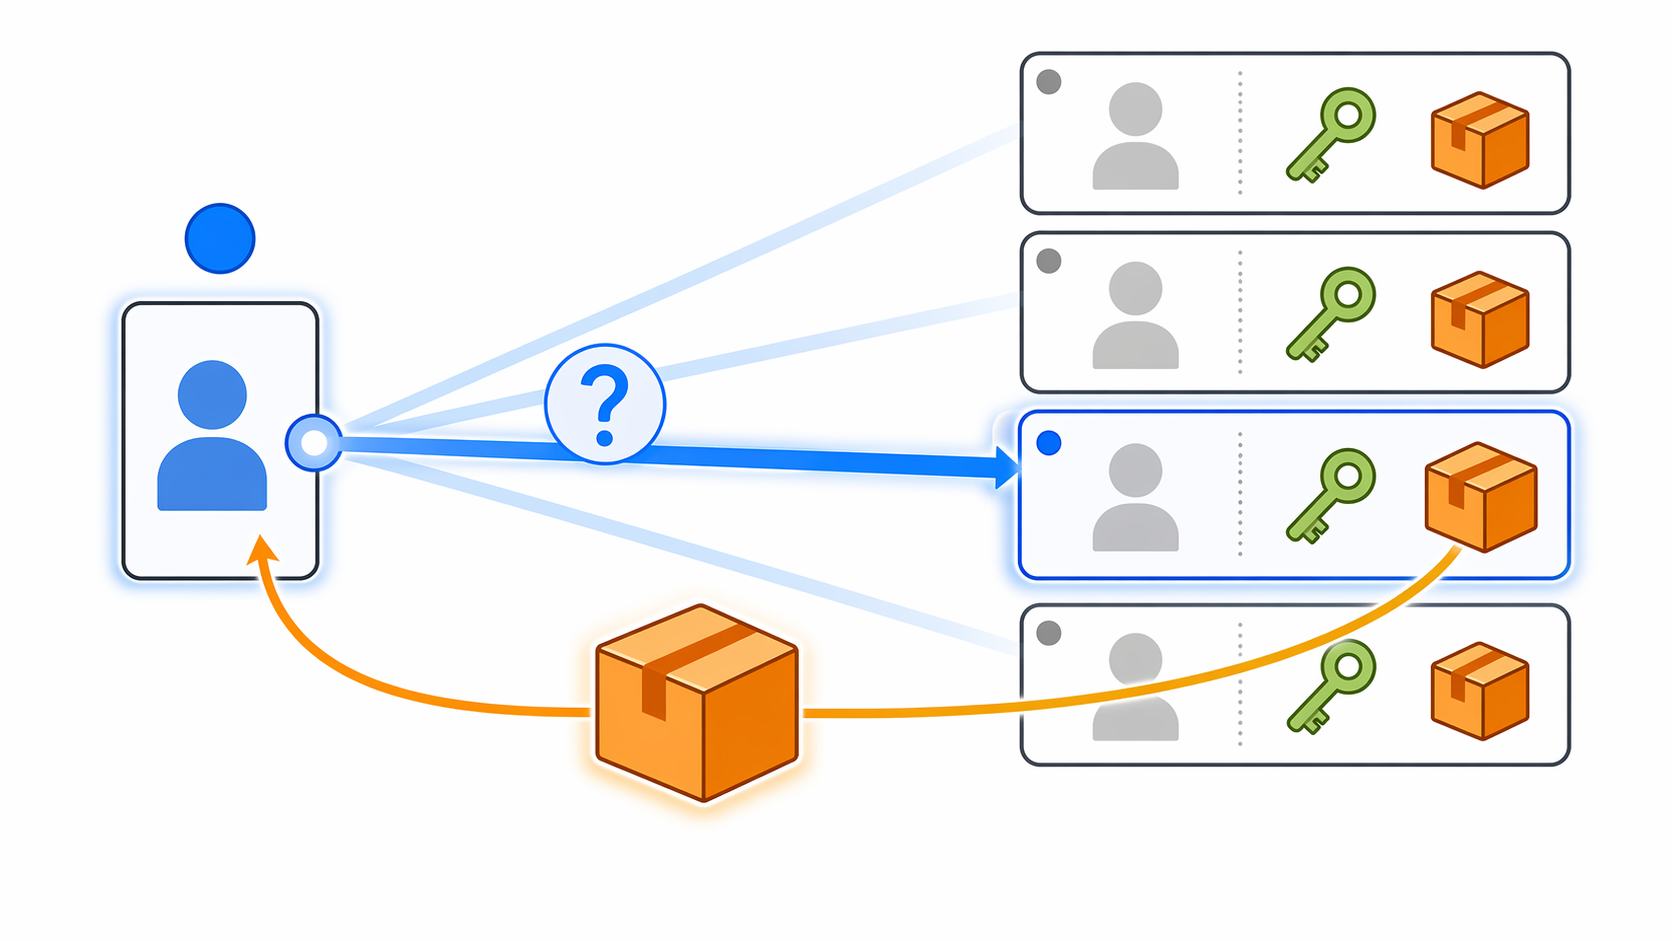
\includegraphics[width=0.92\linewidth]{qkv_roles.png}
  \caption{Query、Key、Value 的角色隐喻：左边 token 发出查询；右侧 token 用 key 参与匹配；匹配强的位置把 value 信息贡献回来。}
  \label{fig:qkv-roles}
\end{figure}

三者的分工如下：

\begin{center}
\begin{tabular}{>{\centering\arraybackslash}p{0.18\linewidth} >{\raggedright\arraybackslash}p{0.67\linewidth}}
\toprule
角色 & 人话解释 \\
\midrule
Query \(Q\) & “我现在想找什么信息？”它属于正在更新自己的 token。\\
Key \(K\) & “我这里有什么信息可供匹配？”它属于被查看的候选 token。\\
Value \(V\) & “如果你决定看我，我实际给你什么内容？”它是最终被加权汇总的信息。\\
\bottomrule
\end{tabular}
\end{center}

这正对应原网页的小节：query 用来询问信息，key 用来响应并计算权重，value 用来贡献最终输出。

\section{Q4：公式每一项是什么意思}

\begin{questionblock}
很多教材直接写：
\[
  \operatorname{Attention}(Q,K,V)
  = \softmax\!\left(\frac{QK^\top}{\sqrt{d_k}}\right)V.
\]
这串符号到底在说什么？
\end{questionblock}

先从单个 token 说起。
假设第 \(i\) 个 token 的输入向量是 \(\vect{x}_i\)。
模型会用三个可训练矩阵把它变成三种角色：

\begin{mathblock}{从一个 token 到三种角色}
\[
  \vect{q}_i = \vect{x}_i W_Q,
  \qquad
  \vect{k}_i = \vect{x}_i W_K,
  \qquad
  \vect{v}_i = \vect{x}_i W_V.
\]
这里 \(\vect{q}_i\) 是第 \(i\) 个 token 的 query 向量，
\(\vect{k}_i\) 是它的 key 向量，
\(\vect{v}_i\) 是它的 value 向量。
\(W_Q,W_K,W_V\) 是训练学出来的矩阵。
\end{mathblock}

\Needspace{7\baselineskip}
接着，第 \(i\) 个 token 要决定看第 \(j\) 个 token 多少，就比较：

\[
  \vect{q}_i \cdot \vect{k}_j.
\]

这句话的人话版本是：
\textbf{第 \(i\) 个 token 的问题，和第 \(j\) 个 token 展示出来的索引标签，有多匹配？}

\begin{mathblock}{缩放点积注意力}
\[
  \alpha_{ij}
  =
  \softmax_j\!\left(
    \frac{\vect{q}_i \cdot \vect{k}_j}{\sqrt{d_k}}
  \right),
  \qquad
  \vect{z}_i = \sum_{j=1}^{n}\alpha_{ij}\vect{v}_j.
\]
\(\alpha_{ij}\) 是第 \(i\) 个 token 分给第 \(j\) 个 token 的注意力权重。
\(d_k\) 是 key/query 向量的维度。
\(\vect{z}_i\) 是第 \(i\) 个 token 更新后的上下文向量。
\end{mathblock}

把所有 token 一次性堆成矩阵，就得到常见公式：

\begin{mathblock}{矩阵形式}
\[
  Q=XW_Q,\qquad K=XW_K,\qquad V=XW_V,
\]
\[
  \boxed{
  \operatorname{Attention}(Q,K,V)
  =
  \softmax\!\left(\frac{QK^\top}{\sqrt{d_k}}\right)V
  }.
\]
其中 \(X\) 是一整句话的输入矩阵；
\(QK^\top\) 是所有 token 两两之间的匹配分数表；
\(\softmax(\cdot)\) 把每一行分数变成权重；
最后乘 \(V\)，就是把 value 信息按权重汇总。
\end{mathblock}

\subsection*{为什么要除以 \(\sqrt{d_k}\)}

\begin{intuitionblock}
点积是很多项相加。
向量维度 \(d_k\) 越大，点积数值越容易变大。
如果分数太大，softmax 会变得非常尖锐：最大的那个位置几乎拿走全部权重。
除以 \(\sqrt{d_k}\) 是为了把分数压回温和范围，让模型保持“软选择”。
\end{intuitionblock}

\section{把一个最小例子走完}

假设一句话有 4 个 token，每个 token 的隐藏维度是 3：

\[
X \in \mathbb{R}^{4\times 3}.
\]

再假设这一层把 query/key/value 都投影到 2 维：

\[
W_Q,W_K,W_V \in \mathbb{R}^{3\times 2}.
\]

那么形状会这样变化：

\begin{center}
\resizebox{\linewidth}{!}{%
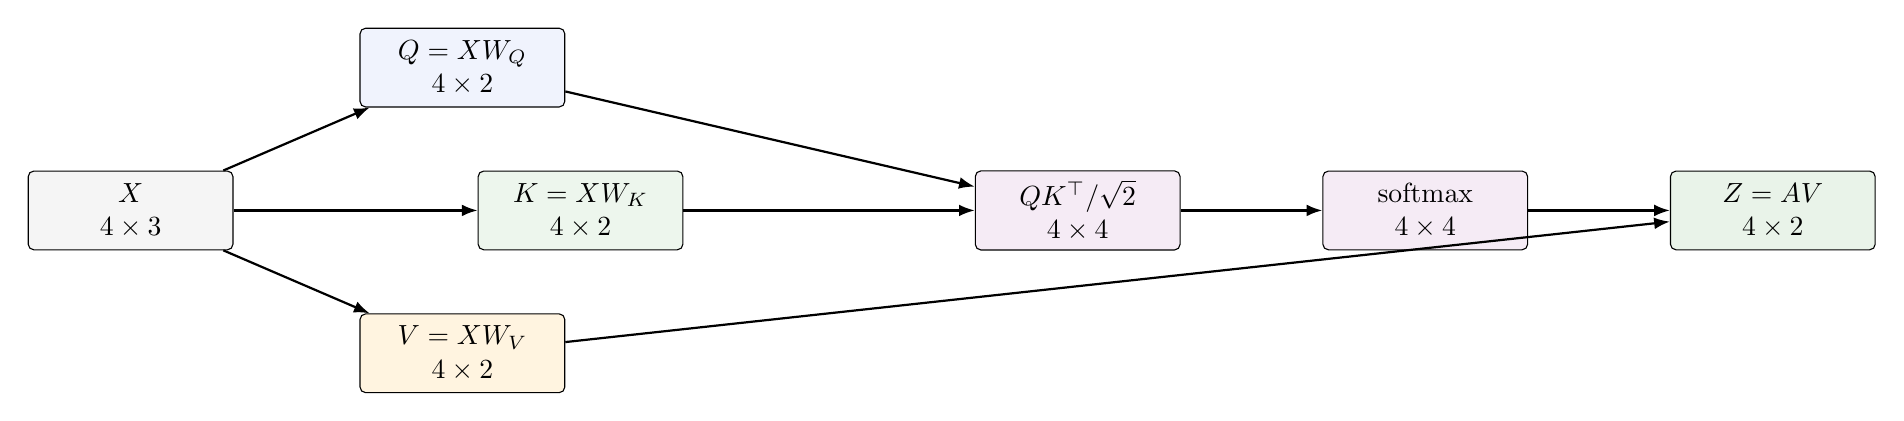
\begin{tikzpicture}[
  node distance=11mm,
  box/.style={draw, rounded corners=2pt, minimum width=26mm, minimum height=10mm, align=center, fill=white},
  op/.style={draw, circle, minimum size=8mm, fill=RoyalBlue!8},
  arr/.style={-{Latex[length=2mm]}, thick}
]
  \node[box, fill=gray!8] (x) {\(X\)\\\(4\times3\)};
  \node[box, fill=RoyalBlue!8, above right=8mm and 16mm of x] (q) {\(Q=XW_Q\)\\\(4\times2\)};
  \node[box, fill=ForestGreen!8, right=31mm of x] (k) {\(K=XW_K\)\\\(4\times2\)};
  \node[box, fill=Orange!12, below right=8mm and 16mm of x] (v) {\(V=XW_V\)\\\(4\times2\)};
  \node[box, fill=Purple!8, right=37mm of k] (scores) {\(QK^\top/\sqrt{2}\)\\\(4\times4\)};
  \node[box, fill=Purple!8, right=18mm of scores] (weights) {softmax\\\(4\times4\)};
  \node[box, fill=ForestGreen!10, right=18mm of weights] (z) {\(Z=AV\)\\\(4\times2\)};

  \draw[arr] (x) -- (q);
  \draw[arr] (x) -- (k);
  \draw[arr] (x) -- (v);
  \draw[arr] (q) -- (scores);
  \draw[arr] (k) -- (scores);
  \draw[arr] (scores) -- (weights);
  \draw[arr] (weights) -- (z);
  \draw[arr] (v) -- (z);
\end{tikzpicture}
}
\end{center}

\begin{keypointblock}
\(4\times4\) 的注意力权重矩阵 \(A\) 最容易误解。
它不是输出本身，而是一张“谁看谁多少”的表。
真正的新 token 表示是 \(Z=AV\)。
\end{keypointblock}

\section{代码里每一步对应什么}

下面是一段简化 PyTorch 代码。
它不追求完整工程结构，只帮助你把公式对回代码。

\begin{codeblock}
\begin{lstlisting}
import torch
import torch.nn as nn

class SelfAttention(nn.Module):
    def __init__(self, d_in, d_k):
        super().__init__()
        self.W_q = nn.Linear(d_in, d_k, bias=False)
        self.W_k = nn.Linear(d_in, d_k, bias=False)
        self.W_v = nn.Linear(d_in, d_k, bias=False)

    def forward(self, x):
        # x: (batch, seq_len, d_in)
        Q = self.W_q(x)  # (batch, seq_len, d_k)
        K = self.W_k(x)  # (batch, seq_len, d_k)
        V = self.W_v(x)  # (batch, seq_len, d_k)

        scores = Q @ K.transpose(-2, -1)      # (batch, seq_len, seq_len)
        scores = scores / (K.shape[-1] ** 0.5)
        weights = torch.softmax(scores, dim=-1)

        out = weights @ V                     # (batch, seq_len, d_k)
        return out, weights
\end{lstlisting}
\end{codeblock}

逐行对照：

\begin{enumerate}
  \item \texttt{W\_q/W\_k/W\_v} 对应 \(W_Q,W_K,W_V\)，是模型要学习的参数。
  \item \texttt{scores} 对应 \(QK^\top\)，表示每个 token 对每个 token 的匹配分数。
  \item \texttt{softmax(scores, dim=-1)} 表示每一行单独归一化：每个查询 token 都有自己的一排注意力权重。
  \item \texttt{weights @ V} 对应最后的加权汇总。
\end{enumerate}

\section{这一节和真实模型还差什么}

到这里，我们只解释了 self-attention 的核心。
真实 Transformer 还会继续加几层东西：

\begin{enumerate}
  \item \textbf{Masked self-attention}：decoder 生成文本时不能偷看未来 token，所以会把未来位置遮住。
  \item \textbf{Multi-head attention}：不是只用一套 Q/K/V，而是分成多个头，让不同头关注不同关系。
  \item \textbf{残差连接和 LayerNorm}：帮助深层网络稳定训练。
  \item \textbf{前馈网络}：attention 负责混合 token 之间的信息，前馈网络负责进一步变换每个位置的表示。
\end{enumerate}

\begin{keypointblock}
本节目标不是把 Transformer 全部讲完。
本节只要拿下一个核心句子：
\textbf{self-attention 让同一句话内部的 token 用 Q/K 匹配权重，再用这些权重汇总 V，从而更新每个 token 自己。}
\end{keypointblock}

\section{一页复盘}

\begin{center}
\begin{tabular}{>{\raggedright\arraybackslash}p{0.23\linewidth} >{\raggedright\arraybackslash}p{0.64\linewidth}}
\toprule
关键词 & 应该记住的人话版本 \\
\midrule
Self-attention & 同一组 token 表示内部互相看。\\
Query & 当前 token 想找什么。\\
Key & 候选 token 怎样被匹配到。\\
Value & 候选 token 真正贡献的信息。\\
\(QK^\top\) & 所有 token 两两之间的匹配分数表。\\
softmax & 把分数变成一排“加起来等于 1”的权重。\\
\(\softmax(QK^\top/\sqrt{d_k})V\) & 先决定看谁多少，再按权重把 value 汇总回来。\\
\bottomrule
\end{tabular}
\end{center}

\begin{keypointblock}
不要把 attention 想成一个神秘模块。
它就是三步：\textbf{算相关分数，变成权重，加权汇总信息}。
Query、Key、Value 只是让这三步变得可学习、可训练。
\end{keypointblock}

\end{document}
